\documentclass[10pt]{article}

\usepackage[margin=0.75in]{geometry}
\usepackage{amsmath,amsthm,amssymb}
\usepackage{xcolor}
\usepackage{cancel}
\usepackage{graphicx}
\usepackage{changepage}
\usepackage{circuitikz}
\usepackage{pgfplots}
\usepackage{physics}
\usepackage{hyperref}
\usepackage{siunitx}
\usepackage{fontspec}
\usepackage{relsize}
\usepackage{subfig}
\usepackage{todonotes}
\usepackage{sagetex}
\usepackage{multicol, multirow, booktabs}
\usepackage[breakable]{tcolorbox}
\usepackage[inline]{enumitem}

\theoremstyle{definition}
\newtheorem{problem}{Problem}
\newtheorem{soln}{Solution}
\makeatletter
\newenvironment{subtheorem}[1]{%
  \def\subtheoremcounter{#1}%
  \refstepcounter{#1}%
  \protected@edef\theparentnumber{\csname the#1\endcsname}%
  \setcounter{parentnumber}{\value{#1}}%
  \setcounter{#1}{0}%
  \expandafter\def\csname the#1\endcsname{\theparentnumber.\Alph{#1}}%
  \ignorespaces
}{%
  \setcounter{\subtheoremcounter}{\value{parentnumber}}%
  \ignorespacesafterend
}
\makeatother
\newcounter{parentnumber}

\pgfplotsset{compat=newest}
\usetikzlibrary{lindenmayersystems}
\usetikzlibrary{arrows}
\usetikzlibrary{calc}
\usetikzlibrary{positioning, fit}
\usetikzlibrary{3d, perspective}
\usetikzlibrary{patterns.meta}

\definecolor{incolor}{HTML}{303F9F}
\definecolor{outcolor}{HTML}{D84315}
\definecolor{cellborder}{HTML}{CFCFCF}
\definecolor{cellbackground}{HTML}{F7F7F7}
\newcommand{\ui}{\hat{i}}
\newcommand{\uj}{\hat{j}}
\newcommand{\uk}{\hat{k}}
\newcommand{\ux}{\hat{x}}
\newcommand{\uy}{\hat{y}}
\newcommand{\uz}{\hat{z}}
\newcommand{\primed}[1]{#1^\prime}
\pgfdeclarelayer{background}  
\pgfsetlayers{background,main}
\AtBeginDocument{\RenewCommandCopy\qty\SI}
\newcommand{\justif}[2]{&{#1}&\text{#2}}
\DeclareMathOperator\Arg{Arg}

\makeatletter
\newcommand{\boxspacing}{\kern\kvtcb@left@rule\kern\kvtcb@boxsep}
\makeatother
\newcommand{\prompt}[4]{
    \ttfamily\llap{{\color{#2}[#3]:\hspace{3pt}#4}}\vspace{-\baselineskip}
}

\newcommand{\thevenin}[2]{
  \begin{center}
    \begin{circuitikz} \draw
      (0,0) -- (2,0) to[battery1, l_=$V_{Th}\eq#1$] (2,2) 
      to[resistor, l_=$R_{Th}\eq#2$] (0,2)
      ;
      \draw [o-] (-.07,2.079);
      \draw [o-] (-.07,0.079);
    \end{circuitikz}
  \end{center}
}

\newcommand{\norton}[2]{
  \begin{center}
    \begin{circuitikz} \draw
      (0,0) -- (3,0) to[american current source, l_=$I_{N}\eq#1$] (3,2) -- (0,2) (2,0)
      to[resistor, l=$R_{N}\eq#2$] (2,2)
      ;
      \draw [o-] (-.07,2.079);
      \draw [o-] (-.07,0.079);
    \end{circuitikz}
  \end{center}
}

\newcommand{\highlight}[1]{\colorbox{yellow}{$\displaystyle #1$}}

\newcommand{\ti}[1]{\widetilde{#1}}

\newfontface{\Kaufmann}{Kaufmann}
\DeclareTextFontCommand{\kf}{\Kaufmann}
\newcommand{\scriptr}{\fontsize{12pt}{12pt}\kf{r}}

\newfontface{\KaufmannB}{Kaufmann Bd BT}
\DeclareTextFontCommand{\kfb}{\KaufmannB}
\newcommand{\bscriptr}{\fontsize{12pt}{12pt}\kfb{r}}

\newcommand{\bv}[1]{\mathbf{#1}}

\title{Math 3770H: Assignment II}
\author{Jeremy Favro (0805980) \\ Trent University, Peterborough, ON, Canada}
\date{\today}

\begin{document}
\maketitle

% PROBLEM 1
\begin{problem}
Write the function
$$f(z)=z+\frac{1}{z}\qquad(z\neq 0)$$
in the form $f(z)=u(r,\theta)+iv(r,\theta)$
\end{problem}
\begin{soln}
  Writing $f$ first in polar form to switch to a dependence on $r=\abs{z},\theta=\arctan\left(\Im z/\Re z\right)$,
  $$z=re^{i\theta}=r\cos\theta+ir\sin\theta.$$
  This is actually really nice here as it means we can easily write the inverse without using a fraction,
  $$z^{-1}=r^{-1}e^{-i\theta}=r^{-1}\cos\left(-\theta\right)+ir^{-1}\sin\left(-\theta\right).$$
  Which can be reworked further using the even/odd nature of $\cos$ and $\sin$ respectively giving:
  \begin{align*}
    f(z) & =r\cos\theta+ir\sin\theta + r^{-1}\cos\theta-ir^{-1}\sin\theta      \\
         & =r\cos\theta+r^{-1}\cos\theta + ir\sin\theta -ir^{-1}\sin\theta     \\
         & =\left(r+r^{-1}\right)\cos\theta +  \left(r+r^{-1}\right)\sin\theta
  \end{align*}
\end{soln}
\newpage

% PROBLEM 2
\begin{problem}
Sketch the region onto which the sector $r \leq 1$, $0 \leq \theta \leq \pi/4$ is mapped by the transformation
\begin{center}
  \begin{enumerate*}[label=(\alph*)]
    \item $w = z^2$;\qquad~
    \item $w = z^3$;\qquad~
    \item $w = z^4$.
  \end{enumerate*}
\end{center}
\end{problem}
\begin{soln}
  Generally the transform $w=z^n$ will give $w=r^ne^{in\theta}$, just by exponentiation laws. Our original region looks like:
  \begin{center}
    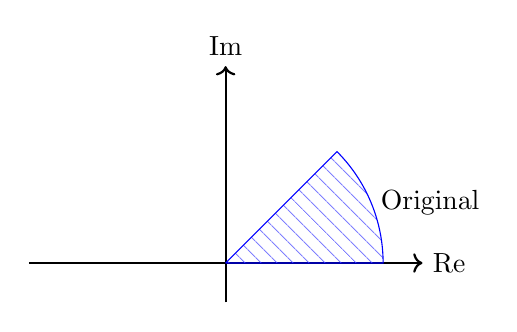
\begin{tikzpicture}[scale=2]
      \draw[->,thick] (-1.25,0)--(1.25,0) node[right]{$\Re$};
      \draw[->,thick] (0,-.25)--(0,1.25) node[above]{$\Im$};
      \filldraw[pattern={Lines[angle=-45,distance=4pt]}, draw=blue, pattern color=blue!50!white] (0,0) -- (1,0) arc (0:45:1) node[midway, right]{Original} -- (0,0);
    \end{tikzpicture}
  \end{center}
  Because our region only extends out to $r=1$ the radius won't change.
  \begin{enumerate}[label=(\alph*)]
    \item ~\begin{center}
            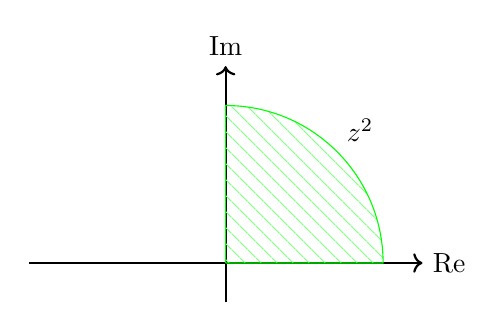
\begin{tikzpicture}[scale=2]
              \draw[->,thick] (-1.25,0)--(1.25,0) node[right]{$\Re$};
              \draw[->,thick] (0,-.25)--(0,1.25) node[above]{$\Im$};
              \filldraw[pattern={Lines[angle=-45,distance=4pt]}, draw=green, pattern color=green!50!white] (0,0) -- (1,0) arc (0:{2*45}:1) node[midway, above right]{$z^2$} -- (0,0);
            \end{tikzpicture}
          \end{center}
    \item ~\begin{center}
            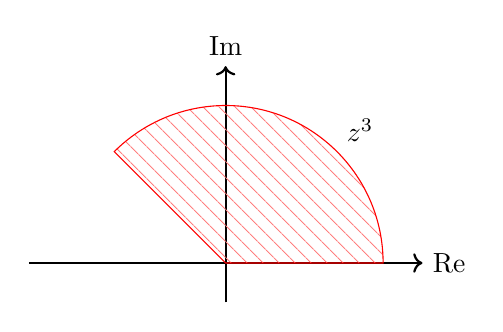
\begin{tikzpicture}[scale=2]
              \draw[->,thick] (-1.25,0)--(1.25,0) node[right]{$\Re$};
              \draw[->,thick] (0,-.25)--(0,1.25) node[above]{$\Im$};
              \filldraw[pattern={Lines[angle=-45,distance=4pt]}, draw=red, pattern color=red!50!white] (0,0) -- (1,0) arc (0:{3*45}:1) node[pos=0.333, above right]{$z^3$} -- (0,0);
            \end{tikzpicture}
          \end{center}
    \item ~\begin{center}
            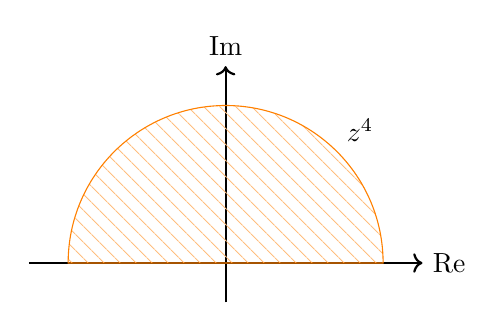
\begin{tikzpicture}[scale=2]
              \draw[->,thick] (-1.25,0)--(1.25,0) node[right]{$\Re$};
              \draw[->,thick] (0,-.25)--(0,1.25) node[above]{$\Im$};
              \filldraw[pattern={Lines[angle=-45,distance=4pt]}, draw=orange, pattern color=orange!50!white] (0,0) -- (1,0) arc (0:{4*45}:1) node[pos=0.25, above right]{$z^4$} -- (0,0);
            \end{tikzpicture}
          \end{center}
  \end{enumerate}
\end{soln}
\newpage

% PROBLEM 3
\begin{problem}
Use definition (2), Sec.15, of the limit to prove that
\begin{center}
  \begin{enumerate*}[label=(\alph*)]
    \item $\lim_{z\to z_0}\Re z = \Re z_0$;\qquad~
    \item $\lim_{z\to z_0}\overline{z}=\overline{z_0}$;\qquad~
    \item $\lim_{z\to 0}\frac{\overline{z}^2}{z}=0$.
  \end{enumerate*}
\end{center}
\end{problem}
\begin{soln}~
  \begin{enumerate}[label=(\alph*)]
    \item Let $\epsilon>0$. Suppose $\abs{z-z_0}<\delta$. If we take $z=x+iy$ and $z_0=x_0+iy_0$ then we have
          $$\abs{\Re z-\Re z_0}=\abs{x-x_0}\leq \abs{z-z_0}.$$
          We can make that last statement because
          $$\abs{x-x_0}\leq \abs{x-x_0+iy-iy_0}=\abs{z-z_0}.$$
          This means that
          $$\abs{\Re z-\Re z_0}=\abs{z-z_0}\leq \delta$$
          by the $\epsilon-\delta$ definition we are using. Having this means that provided
          $\abs{z-z_0}\leq \delta=\epsilon$, then $\abs{\Re z-\Re z_0}<\epsilon$ by transitivity.
    \item Let $\epsilon>0$. Suppose $\abs{z-z_0}<\delta$. We have
          $$\abs{\overline{z}-\overline{z_0}}=\abs{\overline{z-z_0}}=\abs{z-z_0}<\delta$$
          all by properties of the complex conjugate. So provided $\abs{z-z_0}<\delta=\epsilon$, then
          $\abs{\overline{z}-\overline{z_0}}<\epsilon$.
    \item Let $\epsilon>0$. Suppose $\abs{z-z_0}<\delta$. We have
          $$\abs{\frac{\overline{z}^2}{z}-0}=\frac{\abs{\overline{z}^2}}{\abs{z}}=\abs{z}.$$
          This means that $$\abs{\frac{\overline{z}^2}{z}-0}=\abs{z}< \delta=\epsilon$$
  \end{enumerate}
\end{soln}

% PROBLEM 4
\begin{problem}
With the aid of the theorem in Sec. 17, show that when
$$T(z)=\frac{az+b}{cz+d}\qquad (ad-bc)\neq0$$
\begin{enumerate}[label=(\alph*)]
  \item $\lim_{z\to\infty}T(z)=\infty\quad \text{if } c=0$;
  \item $\lim_{z\to\infty}T(z)=\frac{a}{c}\quad\text{and}\quad\lim_{z\to-d/c}T(z)=\infty\quad\text{if } c\neq 0$
\end{enumerate}
\end{problem}
\begin{soln}~
  \begin{enumerate}[label=(\alph*)]
    \item For $c=0$ we get
          $$T(z)=\frac{az+b}{d}.$$
          The referenced theorem states that
          $$\lim_{z\to z_0}T(z)=\infty\quad\text{if}\quad \lim_{z\to z_0}T^{-1}(z)=0.$$
          Here we have then that
          $$\lim_{z\to \infty}T^{-1}(z)=\lim_{z\to \infty}\frac{d}{az+b}=\frac{d}{\infty}=0\implies \lim_{z\to\infty}T(z)=\infty$$
    \item \begin{align*}
             & =\lim_{z\to 0}T(z^{-1})                                                   \\
             & =\lim_{z\to 0}\frac{az^{-1}+b}{cz^{-1}+d}                                 \\
             & =\lim_{z\to 0}\frac{az^{-1}}{cz^{-1}+d}+\cancelto{0}{\frac{b}{cz^{-1}+d}} \\
             & =\lim_{z\to 0}\frac{a}{c\cancelto{1}{zz^{-1}}+\cancelto{0}{dz}}           \\
             & =\frac{a}{c}
          \end{align*}
          Which, by the second part of the given theorem which says that
          $$\lim_{z\to\infty}f(z)=w_0\quad\text{if}\quad\lim_{z\to\infty}f(z^{-1})=w_0$$
          means that our original limit
          $$\lim_{z\to\infty}T(z)=\frac{a}{c}$$
          holds true. For the second part,
          \begin{align*}
             & =\lim_{z\to-d/c}T^{-1}(z)                   \\
             & =\lim_{z\to-d/c}\frac{c(-d/c)+d}{a(-d/c)+b} \\
             & =\lim_{z\to-d/c}\frac{0}{a(-d/c)+b}=0
          \end{align*}
          which by the first part of the theorem (as used in part (a) here) means that our original limit holds true.
  \end{enumerate}
\end{soln}

% PROBLEM 5
\begin{problem}
Use the method in Example 2, Sec. 19, to show that $\primed{f}(z)$ does not exist at any point
$z$ when
\begin{center}
  \begin{enumerate*}[label=(\alph*)]
    \item $f(z)=\Re z$;\qquad~
    \item $f(z)=\Im z$.
  \end{enumerate*}
\end{center}
\end{problem}
\begin{soln}~
  \begin{enumerate}[label=(\alph*)]
    \item $$\frac{\Delta f}{\Delta z}
            =\frac{\Re (z+\Delta z)- \Re z}{\Delta z}
            =\frac{\Re z+\Re \Delta z - \Re z}{\Delta z}
            =\frac{\Re \Delta z}{\Delta z}.$$
          Approaching along the real axis gives $\Delta z=\Delta x+0i$ so
          $$\frac{\Re \Delta z}{\Delta z}=\frac{\Delta x}{\Delta x}=1.$$
          Approaching along the imaginary axis gives $\Delta z = 0+\Delta yi$ so
          $$\frac{\Re \Delta z}{\Delta z}=\frac{0}{\Delta yi}=0.$$
          Because these two do not agree the limit which defines the derivative cannot exist
          and therefore the derivative itself cannot exist.
    \item $$\frac{\Delta f}{\Delta z}
            =\frac{\Im (z+\Delta z)- \Im z}{\Delta z}
            =\frac{\Im z+\Im \Delta z - \Im z}{\Delta z}
            =\frac{\Im \Delta z}{\Delta z}.$$
          We can make the same argument as previously, first approaching along the real axis,
          $$\frac{\Im \Delta z}{\Delta z}=\frac{0}{\Delta x}=0.$$
          Then the imaginary axis,
          $$\frac{\Im \Delta z}{\Delta z}=\frac{\Delta y}{\Delta yi}=-i.$$
          Again because this limit does not exist the derivative cannot exist.
  \end{enumerate}
\end{soln}

% PROBLEM 6
\begin{problem}
Use the theorem in Sec. 24 to show that each of these functions is differentiable in the
indicated domain of definition, and also to find $\primed{f}(z)$:
\begin{enumerate}[label=(\alph*)]
  \item $f(z)=1/z^4$ $(z\neq 0)$;
  \item $f(z)=e^{-\theta}\cos\left(\ln r\right)+ie^{-\theta}\sin\left(\ln r\right)$ $(r>0. 0<\theta<2\pi)$.
\end{enumerate}
\end{problem}
\begin{soln}~
  \begin{enumerate}[label=(\alph*)]
    \item First we note that
          $$f(z)=z^{-4}=r^{-4}\left(\cos\left(4\theta\right)-i\sin\left(4\theta\right)\right).$$
          The partials are then
          \begin{align*}
             & u_r=-4r^{-5}\cos\left(4\theta\right)\qquad u_\theta=-4r^{-4}\sin\left(4\theta\right)  \\
             & v_r=+4r^{-5}\sin\left(4\theta\right)\qquad v_\theta=-4r^{-4}\cos\left(4\theta\right).
          \end{align*}
          These agree with the Cauchy-Riemann equations for polar coordinates,
          $$ru_r=v_\theta\qquad\text{and}\qquad u_\theta=-rv_r$$
          which, alongside the fact that the partials exists for all $(r,\theta)$, satisfies
          the theorem. This means that the derivative will exist for all $(r,\theta)$ in the domain.
          Recalling that, as in real valued functions, the power rule applies, we have that
          $$\primed{f}(x)=-4/z^5.$$
    \item Our partials here are
          \begin{align*}
             & u_r=-r^{-1}e^{-\theta}\sin\left(\ln r\right)\qquad u_\theta=-e^{-\theta}\cos\left(\ln r\right) \\
             & v_r=r^{-1}e^{-\theta}\cos\left(\ln r\right)\qquad v_\theta=-e^{-\theta}\sin\left(\ln r\right).
          \end{align*}
          which satisfy the Cauchy-Riemann equations. Because the trig functions are only undefined (they oscillate infinitely quickly) at $r=0$ which is not
          a part of the domain the derivative exists over the domain.
          Now using the definition of the derivative,
          $$\primed{f}(x)=e^{-i\theta}\left[u_r+iv_r\right]$$
          we get
          $$\primed{f}(x)=e^{-i\theta}\left[-r^{-1}e^{-\theta}\sin\left(\ln r\right)+ir^{-1}e^{-\theta}\cos\left(\ln r\right)\right]$$
  \end{enumerate}
\end{soln}

% PROBLEM 7
\begin{problem}
With the aid of the theorem in Sec. 21, show that each of these functions is nowhere
analytic:
\begin{center}
  \begin{enumerate*}[label=(\alph*)]
    \item $f(z)=xy+iy$;\qquad~
    \item $f(z)=2xy+i(x^2-y^2)$;\qquad~
    \item $f(z)=e^ye^{ix}$.
  \end{enumerate*}
\end{center}
\end{problem}
\begin{soln}~
  \begin{enumerate}[label=(\alph*)]
    \item Here the partials are
          $$u_x=y;\qquad v_y=1;\qquad v_x=0;\qquad u_y=x.$$
          This means that the Cauchy-Riemann equations are
          $$y=1;\qquad x=0.$$
          As the definition for an analytic function requires that the derivative exists on a disk around a point for
          a function to be analytic at the center of the disk, this function cannot be analytic because it is only
          differentiable at $(0,1)$.
    \item Here the partials are
          $$u_x=2y;\qquad v_y=-2y;\qquad v_x=2x;\qquad u_y=2x.$$
          This means that the Cauchy-Riemann equations are
          $$2y=-2y;\qquad 2x=-2x$$
          which implies the derivative only exists at $(0,0)$
          which, by the same reasoning as above, the function is nowhere analytic.
    \item $f(z)=e^ye^{ix}=e^y\left(\cos x i\sin x\right)$
          $$u_x=-e^y\sin x;\qquad v_y=e^y\sin x;\qquad v_x=e^y\cos x;\qquad u_y=e^y\cos x.$$
          This means that the Cauchy-Riemann equations are
          $$-e^y\sin x=e^y\sin x;\qquad e^y\cos x=-e^y\cos x$$
          Which simplifies to
          $$-\sin x=\sin x;\qquad \cos x=-\cos x$$
          which is only true at $x=0$ which is, again, not a neighborhood and this is therefore nowhere analytic.
  \end{enumerate}
\end{soln}

% PROBLEM 8
\begin{subtheorem}{problem}
  \begin{problem}
  Let the function $f (z) = u(x, y) + iv(x, y)$ be analytic in a domain $D$, and consider the
  families of level curves $u(x, y) = c_1$ and $v(x, y) = c_2$, where $c_1$ and $c_2$ are arbitrary
  real constants. Prove that these families are orthogonal. More precisely, show that if
  $z_0 = (x_0,y_0)$ is a point in $D$ which is common to two particular curves $u(x, y) = c_1$
  and $v(x, y) = c_2$ and if $\primed{f}(z_0)\neq0$, then the lines tangent to those curves at $(x_0,y_0)$ are
  perpendicular.
  \end{problem}
  \begin{problem}
  Sketch the families of level curves of the component functions $u$ and $v$ when
  $f(z) = 1/z$, and note the orthogonality described in Exercise 2.
  \end{problem}
\end{subtheorem}
\begin{subtheorem}{soln}
  \begin{soln}
    Coming at this from a multivariate calculus standpoint we know that level curves are orthogonal
    if their normal vectors are orthogonal. These normal vectors are given by the gradient of the corresponding
    function at that point,
    $$\grad{u}=\left(u_x,u_y\right);\qquad \grad{v}=\left(v_x,v_y\right).$$
    For orthogonality we need the inner product,
    $$
      u_xv_x+u_yv_y,
    $$
    to be zero.
    Now as we know that $f(z)$ is analytic we can say that, by definition, the Cauchy-Riemann equations hold in $D$ and
    therefore
    $$u_x=v_y;\qquad u_y=-v_x.$$
    Plugging these into our previous expression for the inner product,
    $$
      v_yv_x-v_xv_y=0.
    $$
  \end{soln}
  \begin{soln}
    With $$f(z)=1/z=1/(x+iy)=\frac{x}{x^2+y^2}-\frac{y}{x^2+y^2}i$$
    we have
    $$u=\frac{x}{x^2+y^2};\qquad v=-\frac{y}{x^2+y^2}$$
    \begin{sagesilent}
      x, y = var('x y')

      f(x,y) = x / (x ^ 2 + y ^ 2)
      f_1(x,y)=-y / (x ^ 2 + y ^ 2)
    \end{sagesilent}
    \begin{center}
      \sageplot[scale=0.5]{contour_plot(lambda x, y: f(x,y), (-1, 1), (-1, 1), contours=[1], fill=False, cmap=['blue'])+contour_plot(lambda x, y: f_1(x,y), (-1, 1), (-1, 1), contours=[1], fill=False, cmap=['green'])}
    \end{center}
Blue: level curve of $u=1$, Green: level curve of $v=1$
  \end{soln}
\end{subtheorem}
\end{document}